% Created 2023-10-19 Thu 14:11
% Intended LaTeX compiler: xelatex
\documentclass[11pt]{tufte-handout}
\usepackage{graphicx}
\usepackage{grffile}
\usepackage{longtable}
\usepackage{wrapfig}
\usepackage{rotating}
\usepackage[normalem]{ulem}
\usepackage{amsmath}
\usepackage{textcomp}
\usepackage{amssymb}
\usepackage{capt-of}
\usepackage[hidelinks]{hyperref}
\usepackage{enumitem}
\setenumerate{itemsep=-3pt,topsep=0pt}
\setitemize{itemsep=-3pt,topsep=0pt}
\usepackage[margin=1in]{geometry}
\author{Roy M. Turner}
\date{Spring, 2021}
\title{A Simple Robot Simulator: simulator.lisp}
\hypersetup{
 pdfauthor={Roy M. Turner},
 pdftitle={A Simple Robot Simulator: simulator.lisp},
 pdfkeywords={},
 pdfsubject={},
 pdfcreator={Emacs 29.0.50 (Org mode 9.6.10)}, 
 pdflang={English}}
\begin{document}

\maketitle
\tableofcontents

\titlepage
\maketitle

\section{Description}
\label{sec:org3175ed4}

This is a very simple ``robot world''  simulator for use by COS 470/570  students for the search assignment. It allows you to define a rectangular world and add some obstacles and one or more robots.  It provides a base class for robots you will define: basically all you have to do is to define a robot class based on \texttt{robot} that has at least the method \texttt{agent-program} that you define to carry out the search program you're interested in; this method will accept a percept in the form described below and provide an action from among the ones defined in \texttt{*commands*}.  You can then use the \texttt{run} function of the simulator to test your agent.  

There are also functions available give you all of the obstacle locations for when you implement your A\textsuperscript{*} search, as well as a very simple function (\texttt{world-sketch}) to show you an overview of the current world.

\section{Loading the simulator}
\label{sec:org0ce29d5}

To load the simulator, make sure that the files \texttt{message.lisp}, \texttt{new-symbol.lisp}, and \texttt{simulator.lisp} are in Lisp's current directory (usually the one you start Lisp in, and the one where your code lives).  Then just do:
\begin{verbatim}
(load "simulator")
\end{verbatim}


The simulator is in its own package, \texttt{simulator}, which has the nickname \texttt{sim}.  Thus you either need to preface all of the simulator-related functions (below) with the package name or nickname, like:
\begin{verbatim}
(sim:create-simulator)
\end{verbatim}

\noindent or import the symbols you are interested in using, e.g.:
\begin{verbatim}
(import '(sim:create-simulator sim:run))
\end{verbatim}

\noindent or import \emph{all} exported symbols from the package:\footnote{Note that although loading \texttt{simulator.lisp} will load the message handler and symbol-creation packages, importing from the \texttt{simulator} package \emph{doesn't} import from those packages.  For that, you will have to do something like \texttt{(use-package 'message)} and \texttt{(use-package 'newsymbol)}.}
\begin{verbatim}
(use-package 'sim)
\end{verbatim}


\textbf{NOTE:} Loading the simulator \emph{also} loads the files \texttt{messages.lisp and =new-symbol.lisp}.  You do not need to load them yourself.  It does \emph{not}, however, import the symbols (functions, methods, etc.) into the \texttt{CL-USER} package the REPL starts in.  To do that, you would need to do, in the REPL or your own files:
\begin{verbatim}
(use-package 'sym)   ;; for the new-symbols file
(use-package 'message) ;; for the messages file
\end{verbatim}


\textbf{NOTE:} As of 2023-10-19, the simulator and associated files no longer spit out the annoying warnings that they did previously. If you want to get rid of similar warnings and style warnings from your own code, you can put the following at the top of your file(s):
\begin{verbatim}
(eval-when (:compile-toplevel :load-toplevel :execute)
  (declaim (sb-ext:muffle-conditions warning))
  (declaim (sb-ext:muffle-conditions style-warning)))
\end{verbatim}
\noindent
and then put this at the bottom to turn them back on after loading:
\begin{verbatim}
(eval-when (:compile-toplevel :load-toplevel :execute)
  (declaim (sb-ext:unmuffle-conditions warning))
  (declaim (sb-ext:unmuffle-conditions style-warning)))
\end{verbatim}



\subsection{If you get an error about package/symbol problems}
\label{sec:org193f514}

Depending on your Lisp, you may already have a symbol in the current package you're using that has the same name as one of the exported (external) symbols in one or more of the other packages you're
importing symbols from, which will result in an error.  For example, with my setup (macOS, SBCL), if I load the ``messages.lisp'' file, then try to \texttt{use-package}, I get this error:

\begin{center}
\begin{center}
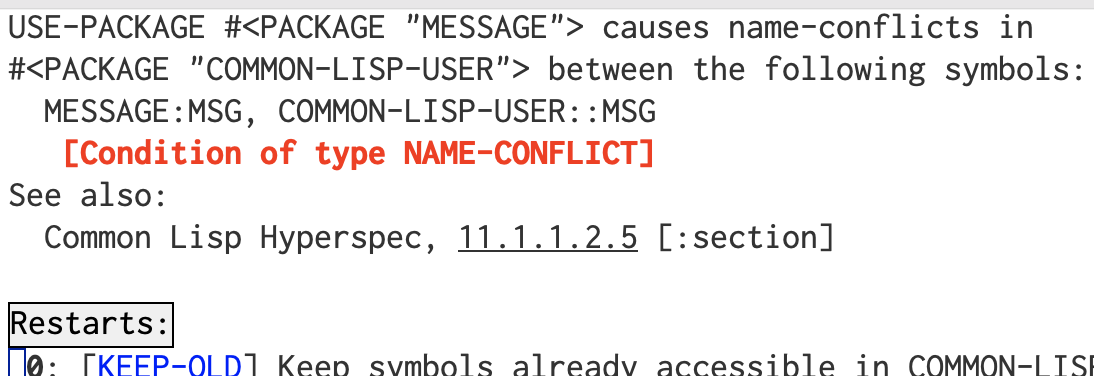
\includegraphics[width=0.7\textwidth]{./Figs/package-error.png}
\end{center}
\end{center}

If this happens, after you load the file you can use \texttt{shadowing-import} to get around this problem.  Suppose that you get an error when calling \texttt{use-package} for the simulator package that tells you the symbol \texttt{name} is in conflict with an existing one in your current package (usually \texttt{cl-user}).  You can fix this by doing the following:
\begin{verbatim}
(shadowing-import 'sim:name)
(use-package sim)
\end{verbatim}


You'll want to make sure that whatever the symbol \texttt{name} had been used for in your current package is not important, though, since you'll no longer be able to access it (except, perhaps, as \texttt{cl-user::name}).  If it was important, you probably want to change to a different name for it.

\section{Creating a simulator}
\label{sec:org0e10dd8}

In order to create a new simulator, you use the \texttt{create-simulator} function, which has the following format:
\begin{verbatim}
create-simulator &key (size '(10 10)) (num-obstacles 0) 
                                    (obstacle-locations nil)
\end{verbatim}

\noindent That is, the default size is 10\texttimes{}10, and no obstacles are added by default when you do:
\begin{verbatim}
(create-simulator)
\end{verbatim}

\noindent You can override these defaults, of course.  To make a different-sized world, e.g.:
\begin{verbatim}
(create-simulator :size '(50 50))
\end{verbatim}

\noindent or to add 10 obstacles:
\begin{verbatim}
(create-simulator :size '(50 50) :num-obstacles 10)
\end{verbatim}


Obstacles created this way will be put in random locations.  If you want to put obstacles in particular places, you can do something like:
\begin{verbatim}
(create-simulator :size '(50 50) 
                            :obstacle-locations '((1 1) (3 4) (10 10)))
\end{verbatim}

\noindent \textbf{Note:} The \((x,y)\) coordinates for the world are 1-based, not 0-based.

You can combine these as well:
\begin{verbatim}
(create-simulator :size '(50 50) :num-obstacles 10 
                            :obstacle-locations '((1 1) (3 4) (10 10)))
\end{verbatim}

\noindent will add 10 random obstacles as well as at the three specified locations.

You will want to put the simulator instance returned by this into a variable, since you'll need it later to do anything:
\begin{verbatim}
(setq sim (create-simulator))
\end{verbatim}

\section{Creating a new robot type}
\label{sec:org9304733}

To run your agent code, you'll need to create a new kind of robot and add it to the simulator.  I have provided a base class for you to use, \texttt{robot}.  The base class has instance variables for the robot's name (\texttt{name}), current location (\texttt{location}), current orientation (\texttt{orientation}, one of \texttt{:north}, \texttt{:south}, \texttt{:east}, or \texttt{:west}), the last percept seen (\texttt{percept}), the next action the agent program has selected (\texttt{next-action}), the previous action (\texttt{prev-action}), and the success status of the previous action (\texttt{prev-action-success}, one of \texttt{t} or \texttt{nil}).

You should not in general, however, access these yourself from your agent program, since these are \emph{simulation} values, not information the agent program knows.  For example, you may want your agent program, for model-based and goal-based agents,  to have and maintain  its own idea of where it is.  This may differ from the real location due to noise or other problems with sensors.  However, for your goal-based agent assignment, where you will be using A\textsuperscript{*} and other search techniques, you may want to just assume no noise and use objects' and the robot's real positions.

You want your agent program---i.e., your AI code---to be run automatically by the simulator at each ``clock tick''.  The simulator is designed to call a \texttt{clock-tick} method of each object (obstacles, robots) for each of its own clock ticks after figuring out what that object should see of the world (i.e., it's percept).  For objects that are not active or are stationary, this is essentially a dummy method.  For a robot class inheriting from the base \texttt{robot} class, the clock tick function calls the class' \texttt{agent-program} method, giving it the current percept. The \texttt{agent-program} method determines what the next action should be and returns it, and the \texttt{clock-tick} both sets the robot's \texttt{next-action} instance variable and returns the next action to its caller.  The simulator's own \texttt{clock-tick} method then continue by calling a method (\texttt{take-action}) to simulate the effect of the robot's \texttt{next-action}.

To run your code, you will need to create another robot class based on \texttt{robot} and define its \texttt{agent-program} method to call your code.  (In fact, you will create a different robot class for each of the parts of the assignment, most likely.)  I have provided a sample robot class, \texttt{random-robot}, that you can look at (below or in \texttt{simulator.lisp}) to see how to do this.

For example, suppose you have written a reflex agent program, named \texttt{reflex} that takes a percept and returns an action to take.  Then all you need to do is:
\begin{verbatim}
(defclass reflex-agent (robot) ())

(defmethod agent-program ((self reflex-agent) percept)
  (reflex percept))
\end{verbatim}

Note that for other kinds of agents, you may need to have a bit more code in \texttt{agent-program} to give your agent program code additional information about the world (e.g., the location of objects in the world).

\subsection{Percept format}
\label{sec:org5567ff9}

For the search assignment, the robots have a very  limited repertoire of sensors: just a forward-looking sonar-type thing that can  sense what is directly in front of the robot and four bump sensors, one on each side and in the front and rear, that can detect whether or not the robot bumped into something due to the \emph{previous} command.  This information is calculated by the simulator's \texttt{clock-tick} method and put into the robot's \texttt{percept} slot just prior to calling the robot's own \texttt{clock-tick} method.

\label{org4949049}

The format of the percept is an \emph{association list}, a list of lists, one for each sensor.  Each list is composed of the sensor name (a symbol) followed by the current value.  The sensors are named \texttt{:front-sensor}, \texttt{:front-bump}, \texttt{:right-bump}, \texttt{:left-bump}, and \texttt{:rear-bump}, each of which will have a value of  \texttt{t} or \texttt{nil} in each percept.  

Here's an example percept:
\begin{verbatim}
((:forward-sensor t)
 (:front-bump nil)
 (:right-bump t)
 (:rear-bump nil)
 (:left-bump nil))
\end{verbatim}

\noindent This would correspond to a situation in which there is something directly in front of the robot, and the last action caused it to bump into something on its right side.\footnote{I know, this is a very verbose and redundant way to provide percepts (for example, no two bump sensors can be \texttt{t} at the same time, etc.), but it easy for you to use.}

Association lists like this are very common in Lisp, especially when you want to have key/value pairs, but don't want a hash table.  There is a special Lisp function, \texttt{assoc}, that is made for interacting with association lists; for example, if \texttt{percept} holds the percept above, then this:
\begin{verbatim}
(assoc :forward-sensor percept)
\end{verbatim}

\noindent will return:
\begin{verbatim}
(forward-sensor t)
\end{verbatim}

\noindent A common idiom, since we just want the value, not the key/value pair, is:
\begin{verbatim}
(cadr (assoc :forward-sensor percept))
\end{verbatim}

\noindent or
\begin{verbatim}
(first (assoc :forward-sensor percept))
\end{verbatim}

\noindent You can set a value in an association list using \texttt{setf}, e.g.,
\begin{verbatim}
(setf (assoc :forward-sensor percept) nili)
\end{verbatim}

\noindent would result in \texttt{percept} having  the value:
\begin{verbatim}
((:forward-sensor nil)
 (:front-bump nil)
 (:right-bump t)
 (:rear-bump nil)
 (:left-bump nil))
\end{verbatim}


You may be wondering what is going on with those colons, and why something like
\begin{verbatim}
(assoc :forward-sensor percept)
\end{verbatim}

\noindent doesn't give an unbound variable error, since \texttt{:forward-sensor} isn't quoted.  Recall that all symbols are contained in \emph{packages}, such as \texttt{cl-user}, \texttt{sim}, etc.  There is a special package, \texttt{keyword}, that has no displayed name, and so if you see a symbol like \texttt{:forward-sensor} with a colon but no name before it, it is a keyword.  Symbols in the \texttt{keyword} package have the very useful property that they all evaluate to themselves.  So you can get something like this:
\begin{verbatim}
CL-USER> :this-is-a-keyword
:THIS-IS-A-KEYWORD
CL-USER>
\end{verbatim}

\noindent whereas if you had done that with a symbol of any other package, you would have gotten an error.

\subsection{Adding new percept components}
\label{sec:orgef868e9}
\label{orge6509b9}

You can add new percept components to robots you define based on \texttt{robot}.  The \texttt{robot} class has an instance variable, \texttt{percept-map}, that contains an association list with elements of the form:
\begin{verbatim}
(sensor-name method)
\end{verbatim}

\noindent where \texttt{sensor-name} is a keyword that names the sensor---and that will show up in the percept---and \texttt{method} is the method to use to compute its value.  The method, which is called by \texttt{calculate-percept} (see the \hyperref[orge28bcd1]{code} below), must take two arguments, a simulator instance and a robot (or your derived, \texttt{robot}-based class), and it needs to return the sensor's value.  You can either specify the sensors you want directly in your robot class' \texttt{percept-map} variable, or you can just add it to the global variable \texttt{*robot-percept-map*}, since \texttt{robot} itself sets its \texttt{percept-map} to that value.

If you do the latter, though, \emph{don't} list a value for \texttt{percept-map} in your class definition!  That will override \texttt{robot}'s.  You're better off, actually,  not listing \texttt{percept-map} among the variables you define for your class unless you \emph{do} want to override the default value.

\subsection{Adding new actions}
\label{sec:org928d1a1}

You may also want to add actions for the robot that are not provided by the standard \texttt{robot} class.  Actions are carried out according to the \texttt{command-map} instance variable of the robot; as you can see from the code, this is set for \texttt{robot} to be the value of the global variable \texttt{*robot-command-map*}.  A command map should be an association list (see \hyperref[org4949049]{above}) whose elements are of the form:
\begin{verbatim}
(cmd method)
\end{verbatim}

\noindent where \texttt{cmd} is the name of the action (or command) your agent program specifies when it returns and \texttt{method} is  a method to carry out the command.  This method needs to accept two arguments, an instance of \texttt{simulator} and an instance of \texttt{robot} (including your \texttt{robot}-derived class); it should return \texttt{t} if it succeeds and \texttt{nil} if not.  These methods are called by the \texttt{take-action} method (see the code below).

You can add your own action/method pairs to \texttt{*robot-command-map*} when you define your robot classes, if you like, since they will inherit from \texttt{robot}, which uses the value of the variable when instantiated as its own internal command map.   You can also define your own in your robot class.


\section{Adding your robot to the simulator}
\label{sec:org61cde99}

Suppose we have the \texttt{reflex-agent} as defined above.  To add an instance of it to the world at a random location, we can just do this (assuming \texttt{sim} contains a simulator instance):
\begin{verbatim}
(add-robot sim :type 'reflex-agent)
\end{verbatim}

\noindent This will create a new instance of \texttt{reflex-agent} for you.  You can instead specify an existing instance by:
\begin{verbatim}
(add-robot sim :robot my-robot)
\end{verbatim}


The \texttt{add-robot} method has additional parameters to allow setting the location (\texttt{:location}), orientation (\texttt{:orientation}), and name (\texttt{:name}, which defaults to a new symbol based on \texttt{robot}).

\section{Changing the world}
\label{sec:orgbff2443}

There are various methods that you can use to change the world.  For example, you can add an object (\texttt{add-object}), find an object (\texttt{find-object}), delete an object (\texttt{remove-object}), clear the entire world while leaving the simulator state alone (\texttt{clear}), and reset the simulator completely (\texttt{reset-simulator}, although why not just create a new instance?).  See the definitions below.

\section{Simulating your work}
\label{sec:org865ee33}

The major function to use to run your simulation is just \texttt{run}.  Original, no?  This has two parameters, both keyword (and thus optional):
\begin{itemize}
\item \texttt{:for} -- how many clock-ticks to run for
\item \texttt{:sketch-each} -- show the state of the world after each clock tick
\end{itemize}
So if you want to run it for 10 seconds (if that's what you want  clock-ticks to be):
\begin{verbatim}
(run sim :for 10 :sketch-each t)
\end{verbatim}


With my random robot example, doing this will give:
\begin{verbatim}
SIM> (run s :for 10 :sketch-each t)
ROBOT0: Moving to (8 2).
++++++++++++
+.......@.@+
+.........@+
+..........+
+......@...+
+@.........+
+....@.....+
+..........+
+@.@.@.....+
+.......>..+
+..@.......+
++++++++++++
ROBOT0: Moving to (9 2).
++++++++++++
+.......@.@+
+.........@+
+..........+
+......@...+
+@.........+
+....@.....+
+..........+
+@.@.@.....+
+........>.+
+..@.......+
++++++++++++
ROBOT0: Turning right, new orientation = :NORTH.
++++++++++++
+.......@.@+
+.........@+
+..........+
+......@...+
+@.........+
+....@.....+
+..........+
+@.@.@.....+
+........^.+
+..@.......+
++++++++++++
++++++++++++
+.......@.@+
+.........@+
+..........+
+......@...+
+@.........+
+....@.....+
+..........+
+@.@.@.....+
+........^.+
+..@.......+
++++++++++++
ROBOT0: Moving to (9 3).
++++++++++++
+.......@.@+
+.........@+
+..........+
+......@...+
+@.........+
+....@.....+
+..........+
+@.@.@...^.+
+..........+
+..@.......+
++++++++++++
ROBOT0: Moving to (8 3).
++++++++++++
+.......@.@+
+.........@+
+..........+
+......@...+
+@.........+
+....@.....+
+..........+
+@.@.@..^..+
+..........+
+..@.......+
++++++++++++
ROBOT0: Moving to (9 3).
++++++++++++
+.......@.@+
+.........@+
+..........+
+......@...+
+@.........+
+....@.....+
+..........+
+@.@.@...^.+
+..........+
+..@.......+
++++++++++++
ROBOT0: Moving to (9 2).
++++++++++++
+.......@.@+
+.........@+
+..........+
+......@...+
+@.........+
+....@.....+
+..........+
+@.@.@.....+
+........^.+
+..@.......+
++++++++++++
ROBOT0: Moving to (8 2).
++++++++++++
+.......@.@+
+.........@+
+..........+
+......@...+
+@.........+
+....@.....+
+..........+
+@.@.@.....+
+.......^..+
+..@.......+
++++++++++++
++++++++++++
+.......@.@+
+.........@+
+..........+
+......@...+
+@.........+
+....@.....+
+..........+
+@.@.@.....+
+.......^..+
+..@.......+
++++++++++++
NIL
SIM> 
\end{verbatim}


I have provided a (very) simple way to show the world, examples of which were just shown.  This is the \texttt{simulator} method \texttt{world-sketch}.  It has keyword arguments that allow you to change what empty characters look like (\texttt{:empty-char}), what the side walls look like (\texttt{:side-wall-char}), and what the top and bottom look like (\texttt{:topo-bottom-char}). 

The character output for each object is obtained by this method by calling each object's \texttt{icon} method, which should return a single character.  The \texttt{robot} version of this outputs a pointer-like symbol to indicate its orientation.


\section{Miscellaneous methods}
\label{sec:orgd6e1fb1}

Here are some additional \texttt{simulator} methods are provided that you may find useful.  I've listed them like you would call them, assuming \texttt{sim} contains a simulator instance.

\begin{itemize}
\item \texttt{(random-location sim)} \(\to\) a random location \texttt{(x y)} in the world
\item \texttt{(random-empty-location sim)} \(\to\) a random location that happens to be empty
\item \texttt{(next-location sim loc dir)} \(\to\) the adjacent location to \texttt{loc} in the direction \texttt{dir}
\item \texttt{(opposite-location sim dir)} \(\to\)  the opposite direction from \texttt{dir}
\item \texttt{(clockwise-direction sim dir)} \(\to\) the direction clockwise from  direction \texttt{dir}
\item \texttt{(counterclockwise-direction sim dir)} \(\to\) the direction counterclockwise from  direction \texttt{dir}
\end{itemize}

And here are some \texttt{world} methods you may find useful; the following assumes \texttt{w} contains an instance of \texttt{world}:
\begin{itemize}
\item (objects w) \(\to\) list of object instances in the world
\item (object-locations w) \(\to\) list of all locations occupied by an object
\item (empty? w loc) \(\to\) \texttt{t} if the location is empty, \texttt{nil} otherwise
\item (in-bounds? w loc) \(\to\) \texttt{t} if location is inside the world, \texttt{nil} otherwise
\item (add-object w object) \(\to\) adds the object (or robot or \ldots{}) instance to the world
\item (clear w) \(\to\) removes all objects from world
\item (size w) \(\to\) size of the world (as two-element list)
\item (delete-object w object), (remove-object w object) \(\to\) (synonyms) remove the object from the world
\item (find-object w x) \(\to\) returns the object if found, \texttt{nil} otherwise; \texttt{x} can be an object (and so will return non-nil if the object is in the world), a location (returns the object at that location), or the name of an object (a symbol)
\item (world-array w) \(\to\) returns an array representing the world, with icons for objects (using the objects'  \texttt{icon} methods) and \texttt{nil} everywhere else; used by \texttt{world-sketch}
\end{itemize}

((export '(objects empty? in-bounds? add-object clear object-locations size delete-object find-objectremove-object world-array))


\section{Code}
\label{sec:org2de34f5}
\label{orge28bcd1}

In the code below, 
I have split up the action of exporting symbols so that you can better see which ones are available to you to import; look for lines that look like:
\begin{verbatim}
(export ...)
\end{verbatim}

\subsection{Muffle warnings and style-warnings}
\label{sec:org9c6593a}
This will get rid of the warnings and style warnings from this file and the others it loads.

\begin{verbatim}
1  (eval-when (:compile-toplevel :load-toplevel :execute)
2    (declaim (sb-ext:muffle-conditions warning))
3    (declaim (sb-ext:muffle-conditions style-warning)))
\end{verbatim}


\subsection{Package setup}
\label{sec:orga90ce01}

Here is the package setup; see above for how to load the package and use it's exported symbols.  As mentioned, this package uses a couple of others, and the \texttt{shadowing-import} function's use is also explained above.

\begin{verbatim}
 4  (unless (find-package "SIM")
 5    (defpackage "SIMULATOR"
 6      (:use "COMMON-LISP")
 7   ;   (:shadowing-import-from "COMMON-LISP" "NAME")
 8      (:nicknames "SIM"))
 9      )
10  
11  (in-package sim)
12  
13  (shadowing-import '(NAME) :cl-user)
14  
15  (load "new-symbol")
16  (use-package 'sym)
17  (load "messages")
18  (shadowing-import 'msg:msg)
19  (use-package 'message)
\end{verbatim}

\subsection{Global variables}
\label{sec:org6d5bad1}

The first of these just lists the directions the simulator/world deals with.  The second is a map (well, an association list) that maps from robot actions (e.g., \texttt{:right}) to methods that carry out those actions (e.g., \texttt{do-move-right}).  The third is a similar map for percepts.  See \hyperref[orge6509b9]{above} for more information about both of them.

\begin{verbatim}
20  (defvar *directions* '(:north :south :east :west))
21  
22  (defvar *robot-command-map*
23      '((:nop do-nop)
24        (:forward do-move-forward)
25        (:backward do-move-backward)
26        (:left do-move-left)
27        (:right do-move-right)
28        (:turn-right do-turn-clockwise)
29        (:turn-left do-turn-counterclockwise)))
30  
31  (defvar *robot-percept-map*
32      '((:front-sensor forward-sensor)
33        (:front-bump front-bump-sensor)
34        (:rear-bump rear-bump-sensor)
35        (:right-bump right-bump-sensor)      
36        (:left-bump left-bump-sensor)))
37  
38  (export '(*robot-command-map* *robot-percept-map* *directions*))
\end{verbatim}

\subsection{Classes}
\label{sec:org30d7381}

Since some classes are referenced by methods of other classes, the classes should be created first.

\begin{verbatim}
39  (defclass simulator ()
40    (
41     (world :initarg :world :initform nil)
42     (time :initarg :time :initform 0)
43     )
44    )
45  
46  (export 'simulator)
47  
48  (defclass world ()
49    (
50     (size :initarg :size :initform '(10 10))
51     (objects :initarg :objects :initform nil)
52     )
53    )
54  
55  (export 'world)
56  
57  (defclass object ()
58    (
59     (name :initarg :name :initform (new-symbol 'o))
60     (location :initarg :location :initform '(1 1))
61     (orientation :initarg :orientation :initform :north)
62      )
63    )
64  
65  (export 'object)
66  
67  (defclass robot (object)
68    (
69     (name :initarg :name :initform (new-symbol 'robot))
70     (percept :initarg :percept :initform nil)
71     (next-action :initarg :next-action :initform :nop)
72     (prev-action :initarg :prev-action :initform nil)
73     (prev-action-success :initarg :prev-action-success :initform nil)
74     (command-map :initarg :command-map
75  		:initform *robot-command-map*)
76     (percept-map :initarg :percept-map
77  		:initform *robot-percept-map*)
78     )
79    )
80  
81  (export 'robot)
\end{verbatim}

\subsection{Simulator methods}
\label{sec:org2c10004}

\begin{verbatim}
 82  (defmethod clear ((self simulator))
 83    (with-slots (world) self
 84      (clear world)))
 85  
 86  (export 'clear)
 87  
 88  (defmethod reset-simulator ((self simulator) &key clear?)
 89    (with-slots (time world) self
 90      (setq time 0)
 91      (when clear?
 92        (clear world))))
 93  
 94  (export 'reset-simulator)
 95  
 96  (defmethod add-obstacles ((self simulator) locations)
 97    (dolist (loc locations)
 98      (add-obstacle self loc)))
 99  
100  (export 'add-obstacles)
\end{verbatim}

This next pair of methods demonstrate CLOS' function polymorphism.  CLOS is a \emph{generic function}-based object-oriented system, unlike, say, in Python or Java, where methods are tightly associated with the classes themselves as part of their definitions.  In CLOS, all methods are instances of some ``generic function'' that when called, checks to see which method is appropriate for its arguments.  The first method below, for example, would be used if:
\begin{verbatim}
(add-obstacle sim foo)
\end{verbatim}

\noindent is called and \texttt{sim} is a simulator instance and \texttt{foo} is an instance of \texttt{object}.  The second would be called otherwise.

These restrictions aren't limited to user-defined objects, either; for example, you can  specify that an argument must be a symbol, number, cons cell, etc.:
\begin{verbatim}
SIM> (defmethod foo ((a number)) nil)
#<STANDARD-METHOD SIMULATOR::FOO (NUMBER) {10047F9B93}>
SIM> (defmethod foo ((a number)) nil)
#<STANDARD-METHOD SIMULATOR::FOO (NUMBER) {10048391F3}>
SIM> (defmethod foo (a) t)
#<STANDARD-METHOD SIMULATOR::FOO (T) {100486CC93}>
SIM> (foo 3)
NIL
SIM> (foo 'a)
T
\end{verbatim}


\begin{verbatim}
101  (defmethod add-obstacle ((self simulator) (object object))
102    (with-slots (world) self
103      (add-object world object)))
104  
105  (defmethod add-obstacle ((self simulator) location)
106    (with-slots (world) self
107      (add-object world (make-instance 'object :name (new-symbol 'obj) :location location))))
108  
109  (export 'add-obstacle)
110  
111  (defmethod add-object ((self simulator) object)
112    (add-obstacle self object))
113  
114  (export 'add-object)
115  
116  (defmethod add-random-obstacles ((self simulator) &key number (max 20) (min 1))
117    (unless number
118      (setq number (random (+ (- max min) 1))))
119    (dotimes (i number)
120      (add-random-obstacle self)))
121  
122  (export 'add-random-obstacles)
123  
124  (defmethod add-random-obstacle ((self simulator))
125    (with-slots (world) self
126      (add-object world (make-instance 'object :location (random-empty-location self)))))
127  
128  (export 'add-random-obstacle)
129  
130  (defmethod add-robot ((self simulator) &key (robot nil) 
131  					    (name (new-symbol 'robot))
132  					    (location (random-empty-location self))
133  					    (orientation (nth (random 4) *directions*))
134  					    (type 'robot))
135    (with-slots (world) self
136      (unless (empty? world location)
137        (error "Can't add a robot to ~s: square is not empty." location))
138      (unless robot
139        (setq robot 
140  	(make-instance type :name name 
141  		       :location location :orientation orientation)))
142      (add-object world robot)
143      robot))
144  
145  (export 'add-robot)
146  
147  (defmethod delete-object ((self simulator) object)
148    (with-slots (world) self
149      (delete-object world object)))
150  
151  (export 'delete-object)
152  
153  (defmethod random-location ((self simulator))
154    (with-slots (world) self
155      (list (+ (random (car (size world))) 1)
156  	  (+ (random (cadr (size world))) 1))))
157  
158  (export 'random-location)
159  
160  (defmethod random-empty-location ((self simulator))
161    (with-slots (world) self
162      (loop with loc
163  	do (setq loc (list (+ (random (car (size world))) 1)
164  			   (+ (random (cadr (size world))) 1)))
165  	until (empty? world loc)
166  	finally (return loc))))
167  
168  (export 'random-empty-location)
169  
170  (defmethod next-location ((self simulator) location direction)
171    (case direction
172      (:north (list (car location) (1+ (cadr location))))
173      (:east (list (1+ (car location)) (cadr location)))
174      (:south (list (car location) (1- (cadr location))))
175      (:west (list (1- (car location)) (cadr location)))))
176  
177  (export 'next-location)
178  
179  (defmethod opposite-direction ((self simulator) direction)
180    (case direction
181      (:north :south)
182      (:south :north)
183      (:east :west)
184      (:west :east)))
185  
186  (export 'opposite-direction)
187  
188  (defmethod clockwise-direction ((self simulator) direction)
189    (case direction
190      (:north :east)
191      (:south :west)
192      (:east :south)
193      (:west :north)))
194  
195  (export 'clockwise-direction)
196  
197  (defmethod counterclockwise-direction ((self simulator) direction)
198    (opposite-direction self (clockwise-direction self direction)))
199  
200  (export 'counterclockwise-direction)
201  
202  (defmethod run ((self simulator) &key (for 1) (sketch-each nil))
203    (dotimes (i for)
204      (clock-tick self)
205      (when sketch-each 
206        (world-sketch self))))
207  
208  (export 'run)
209  
210  (defmethod clock-tick ((self simulator))
211    (with-slots (world time) self
212      (dmsg ".")
213      (dolist (object (objects world))
214        (calculate-percept self object)
215        (clock-tick object)
216        (take-action self object))
217      (incf time)))
218  
219  (defmethod find-object ((self simulator) description)
220    (with-slots (world) self
221      (find-object world description)))
222  
223  (export 'find-object)
224  
225  (defmethod remove-object ((self simulator) description)
226    (with-slots (world) self
227      (remove-object world description)))
228  
229  (export 'remove-object)
230  
231  (defmethod world-sketch ((self simulator) &key (empty-char #\.) (side-wall-char #\+)
232  						(top-bottom-char #\+))
233  
234    (with-slots (world) self
235      (with-slots (size) world
236        (let ((w (world-array world)))
237  	(write side-wall-char :escape nil)
238  	(write (make-string (cadr size) :initial-element top-bottom-char) :escape nil)
239  	(write side-wall-char :escape nil)
240  	(fresh-line)
241  	(loop for j from (1- (car size)) downto 0
242  	    do
243  	      (write side-wall-char :escape nil)
244  	      (dotimes (i (cadr size))
245  		(if (null (aref w i j))
246  		  (write empty-char :escape nil)
247  		  (write (aref w i j) :escape nil)))
248  	      (write side-wall-char :escape nil)
249  	      (fresh-line))
250  	(write side-wall-char :escape nil)
251  	(write (make-string (cadr size) :initial-element top-bottom-char) :escape nil)
252  	(write side-wall-char :escape nil)
253  	(fresh-line)))))
254  
255  (export 'world-sketch)
256  
257  (defun create-simulator (&key (size '(10 10))
258  			      (num-obstacles 0)
259  			      (obstacle-locations nil)
260  			      )
261    (let* ((sim (make-instance 'simulator
262  		:world (make-instance 'world :size size))))
263      (when obstacle-locations
264        (add-obstacles sim obstacle-locations))
265      (unless (zerop num-obstacles)
266        (add-random-obstacles sim :number num-obstacles))
267      sim))
268  
269  (export 'create-simulator)
\end{verbatim}


\begin{enumerate}
\item Sensor methods
\label{sec:org75c16c5}

Percepts are created by the method(s) \texttt{calculate-percept}.  Even though I have put these methods here, as you can see, they are just as much ``methods of'' objects as the simulator.   See the discussion of percepts above for more information.

\begin{verbatim}
270  (defmethod calculate-percept ((self simulator) (object object))
271    )
272  
273  (defmethod calculate-percept ((self simulator) (object robot))
274    (with-slots (time) self
275      (with-slots (name percept-map percept) object
276        (dfmsg "[~s  Calculating percept for ~s]" time name)
277        (setq percept 
278  	(loop for percept in percept-map
279  	    collect (list (car percept)
280  			  (funcall (cadr percept) self object)))))))
281  
282  (defmethod forward-sensor ((self simulator) object)
283    (with-slots (location orientation) object
284      (with-slots (world) self
285        (not (empty? world (next-location self location orientation))))))
286  
287  (defmethod front-bump-sensor ((self simulator) (object robot))
288    (bump-sensor self object :forward))
289  
290  (defmethod rear-bump-sensor ((self simulator) (object robot))
291    (bump-sensor self object :backward))
292  
293  (defmethod left-bump-sensor ((self simulator) (object robot))
294    (bump-sensor self object :left))
295  
296  (defmethod right-bump-sensor ((self simulator) (object robot))
297    (bump-sensor self object :right))
298  
299  (defmethod bump-sensor ((self simulator) object which)
300    (with-slots (location orientation prev-action prev-action-success) object
301      (with-slots (world) self
302        (and
303         (eql prev-action which)
304         (eql nil prev-action-success)
305         (not
306  	(empty? world
307  		(next-location self
308  			       location 
309  			       (case which
310  				 (:forward orientation)
311  				 (:backward
312  				  (opposite-direction self orientation))
313  				 (:left
314  				  (counterclockwise-direction self orientation))
315  				 (:right
316  				  (clockwise-direction self orientation))))))))))
317  
318  (export '(forward-sensor front-bump rear-bump left-bump right-bump bump-sensor))
\end{verbatim}
\item Effector (actuator) methods
\label{sec:orga253c21}

The method \texttt{take-action}, which is specialized for each kind of object, does whatever the \texttt{next-action} of the robot is.  See above for how to add new actions.

Here are the supplied \texttt{take-action} methods:

\begin{verbatim}
319  (defmethod take-action ((self simulator) (object object))
320    (vdfmsg "[~s: ignoring take-action method]" (slot-value object 'name))
321    )
322  
323  (defmethod take-action ((self simulator) (object robot))
324    (with-slots (time) self
325      (with-slots (prev-action prev-action-success next-action
326  		 name command-map) object
327        (let ((command (cadr (assoc next-action command-map))))
328  	(cond
329  	 ((null command)
330  	  (warn "~s  Command ~s isn't implemented for ~s; ignoring." 
331  		time next-action name)
332  	  (setq prev-action-success nil))
333  	 (t
334  	  (fmsg "~s  ~s: Performing action ~s." time name next-action)
335  	  (dfmsg "[~s: calling method ~s]" name command)
336  	  (setq prev-action-success (funcall command self object))
337  	  ))
338  	(setq prev-action next-action)
339  	(setq next-action nil)
340  	prev-action-success))))
341  
342  (defmethod do-nop ((self simulator) (object object))
343    (declare (ignore self object))
344    t)
345  
346  (defmethod do-move-forward ((self simulator) (object object))
347    (with-slots (name location orientation) object
348      (move-object self object (next-location self location orientation))))
349  
350  (defmethod do-move-backward ((self simulator) (object object))
351    (with-slots (name location orientation) object
352      (move-object self object
353  		 (next-location self
354  				location (opposite-direction self orientation)))))
355  
356  (defmethod do-move-left ((self simulator) (object object))
357    (with-slots (name location orientation) object
358      (move-object self object
359  		 (next-location self
360  				location (counterclockwise-direction
361  					  self orientation)))))
362  
363  (defmethod do-move-right ((self simulator) (object object))
364    (with-slots (name location orientation) object
365      (move-object self object
366  		 (next-location self location (clockwise-direction
367  					       self orientation)))))
368  
369  (defmethod do-turn-clockwise ((self simulator) (object object))
370    (turn-object self object :clockwise))
371  
372  (defmethod do-turn-counterclockwise ((self simulator) (object object))
373    (turn-object self object :counterclockwise))
374  
375  
376  (defmethod turn-object ((self simulator) (object object) direction)
377    (declare (ignore direction))
378    t)
379  
380  (defmethod turn-object ((self simulator) (object robot) direction)
381    (with-slots (orientation name) object
382      (setq orientation (if (eql direction :clockwise)
383  			(clockwise-direction self orientation)
384  			(counterclockwise-direction self orientation)))
385      (fmsg "~s: Turning right, new orientation = ~s." 
386  	  name orientation)
387      t))
388  
389  (defmethod move-object ((self simulator) object new-loc)
390    (with-slots (name location) object
391      (with-slots (world) self
392        (cond
393         ((empty? world new-loc)
394  	(setq location new-loc)
395  	(fmsg "~s: Moving to ~s." name location)
396  	t)
397         (t
398  	(fmsg "~s: Tried and failed to move to ~s." name location)
399  	nil)))))
400  
401  (export '(do-nop do-move-forward do-move-backward do-move-left
402  	  do-move-right do-turn-clockwise do-turn-counterclockwise 
403  	  turn-object move-object ))
\end{verbatim}
\end{enumerate}

\subsection{World methods}
\label{sec:orgc1cb60c}

\begin{verbatim}
404  (defmethod objects ((self world))
405    (with-slots (objects) self
406      objects))
407  
408  (defmethod empty? ((self world) location)
409    (with-slots (objects size) self
410        (and (> (car location) 0)
411  	   (<= (car location) (car size))
412  	   (> (cadr location) 0)
413  	   (<= (cadr location) (cadr size))
414  	   (loop for obj in objects
415  	       when (equal (slot-value obj 'location) location)
416  	       return nil
417  	       finally (return t)))))
418  
419  (defmethod in-bounds? ((self world) loc)
420    (with-slots (size) self
421      (and (>= (car loc) 1) (<= (car loc) (car size))
422  	 (>= (cadr loc) 1) (<= (cadr loc) (cadr size)))))
423  
424  (defmethod add-object ((self world) object)
425    (with-slots (size objects) self
426      (with-slots (location name) object
427        (cond
428         ((not (in-bounds? self location))
429  	(cerror "Continue" "Can't add object ~s at ~s -- out of bounds." 
430  	       name location)
431  	nil)
432         ((not (empty? self location))
433  	(cerror "Continue" "Can't add object ~s at ~s -- location isn't empty" 
434  	        name location)
435  	nil)
436         (t (push object objects))))))
437  
438  (defmethod clear ((self world))
439    (with-slots (objects) self
440      (setq objects nil)))
441  
442  (defmethod object-locations ((self world))
443    (with-slots (objects) self
444      (mapcar #'(lambda (o) (copy-list (slot-value o 'location)))
445  	    objects)))
446  
447  (defmethod size ((self world))
448    (with-slots (size) self
449      size))
450  
451  (defmethod delete-object ((self world) object)
452    (remove-object self object))
453  
454  
455  
456  (defmethod remove-object ((self world) description)
457    (with-slots (objects) self
458      (let ((obj (find-object self description)))
459        (when obj
460  	(with-slots (name) obj
461  	  (dfmsg "[Removing object ~s from world]" name)
462  	  (setq objects (remove obj objects)))))))
463  
464  
465  (defmethod find-object ((self world) (location cons))
466    (with-slots (objects) self
467      (car (member location objects :test #'(lambda (a b) 
468  					    (equal a (location b)))))))
469  
470  
471  (defmethod find-object ((self world) (location symbol))
472    (with-slots (objects) self
473      (car (member location objects :test #'(lambda (a b) 
474  					    (eql a (name b)))))))
475  
476  (defmethod find-object ((self world) (object object))
477    (with-slots (objects) self
478      (car (member object objects))))
479  
480  
481  
482  
483  (defmethod world-array ((self world))
484    (with-slots (size objects) self
485      (let ((a (make-array size :initial-element nil)))
486        (dolist (obj objects)
487  	(setf (aref a (1- (car (slot-value obj 'location)))
488  		    (1- (cadr (slot-value obj 'location))))
489  	  (icon obj)))
490        a)))
491  (export '(objects empty? in-bounds? add-object clear object-locations size delete-object find-objectremove-object world-array))
\end{verbatim}

\subsection{Object methods}
\label{sec:org5efd0e1}

\begin{verbatim}
492  (defmethod clock-tick ((self object))
493    :nop)
494  
495  (defmethod name ((self object))
496    (with-slots (name) self
497      name))
498  
499  (export 'name)
500  
501  (defmethod location ((self object))
502    (with-slots (location) self
503      location))
504  
505  (export 'location)
506  
507  (defmethod orientation ((self object))
508    (with-slots (orientation) self
509      orientation))
510  
511  (export 'orientation)
512  
513  (defmethod icon ((self object))
514    #\@)
515  
516  (export 'icon)
\end{verbatim}

\subsection{Robot methods}
\label{sec:orgca11f6c}

\begin{verbatim}
517  (defmethod clock-tick ((self robot))
518    (with-slots (percept next-action name agent-program) self
519      (setq next-action (agent-program self percept))
520      (dfmsg "[~s: ~s -> ~s]" name percept next-action)
521      next-action
522      ))
523  
524  (defmethod agent-program ((self robot) percept)
525    (with-slots (name percept next-action) self
526      (dfmsg "[~s: current percept = ~s, next action = ~s]"
527  	   name percept next-action)
528      (setq next-action :nop)
529      ))
530  
531  (export 'agent-program)
532  
533  
534  (defmethod icon ((self robot))
535    (with-slots (orientation) self
536      (case orientation
537        (:north #\^)
538        (:south #\v)
539        (:east #\>)
540        (:west #\<)
541        (otherwise #\R))))
\end{verbatim}

\subsection{Example: \texttt{random-robot}}
\label{sec:orgab24261}
\begin{verbatim}
542  (defclass random-robot (robot) ())
543  
544  (export 'random-robot)
545  
546  (defmethod agent-program ((self random-robot) percept)
547    (with-slots (name) self 
548      (let ((next-action (car (nth (random (length *robot-command-map*)) 
549  				 *robot-command-map*))))
550        (dfmsg "[~s: percept = ~s]" name percept) 
551        (dfmsg "[~s: choosing ~s as next action]" name next-action)
552        next-action)))
\end{verbatim}

\subsection{Restore the warnings and style warnings:}
\label{sec:org766c1a0}
\begin{verbatim}
553  (eval-when (:compile-toplevel :load-toplevel :execute)
554    (declaim (sb-ext:unmuffle-conditions warning))
555    (declaim (sb-ext:unmuffle-conditions style-warning)))
\end{verbatim}
\end{document}